\documentclass[12pt]{letter}\usepackage[letterpaper,margin=0.65in]{geometry}\usepackage{textcomp}\usepackage{graphicx}\usepackage[rflt]{floatflt}\pagenumbering{gobble}\begin{document}\begin{floatingfigure}{0.15\textwidth}\raisebox{0pt}[0pt][0pt]{\raisebox{-2.5cm}{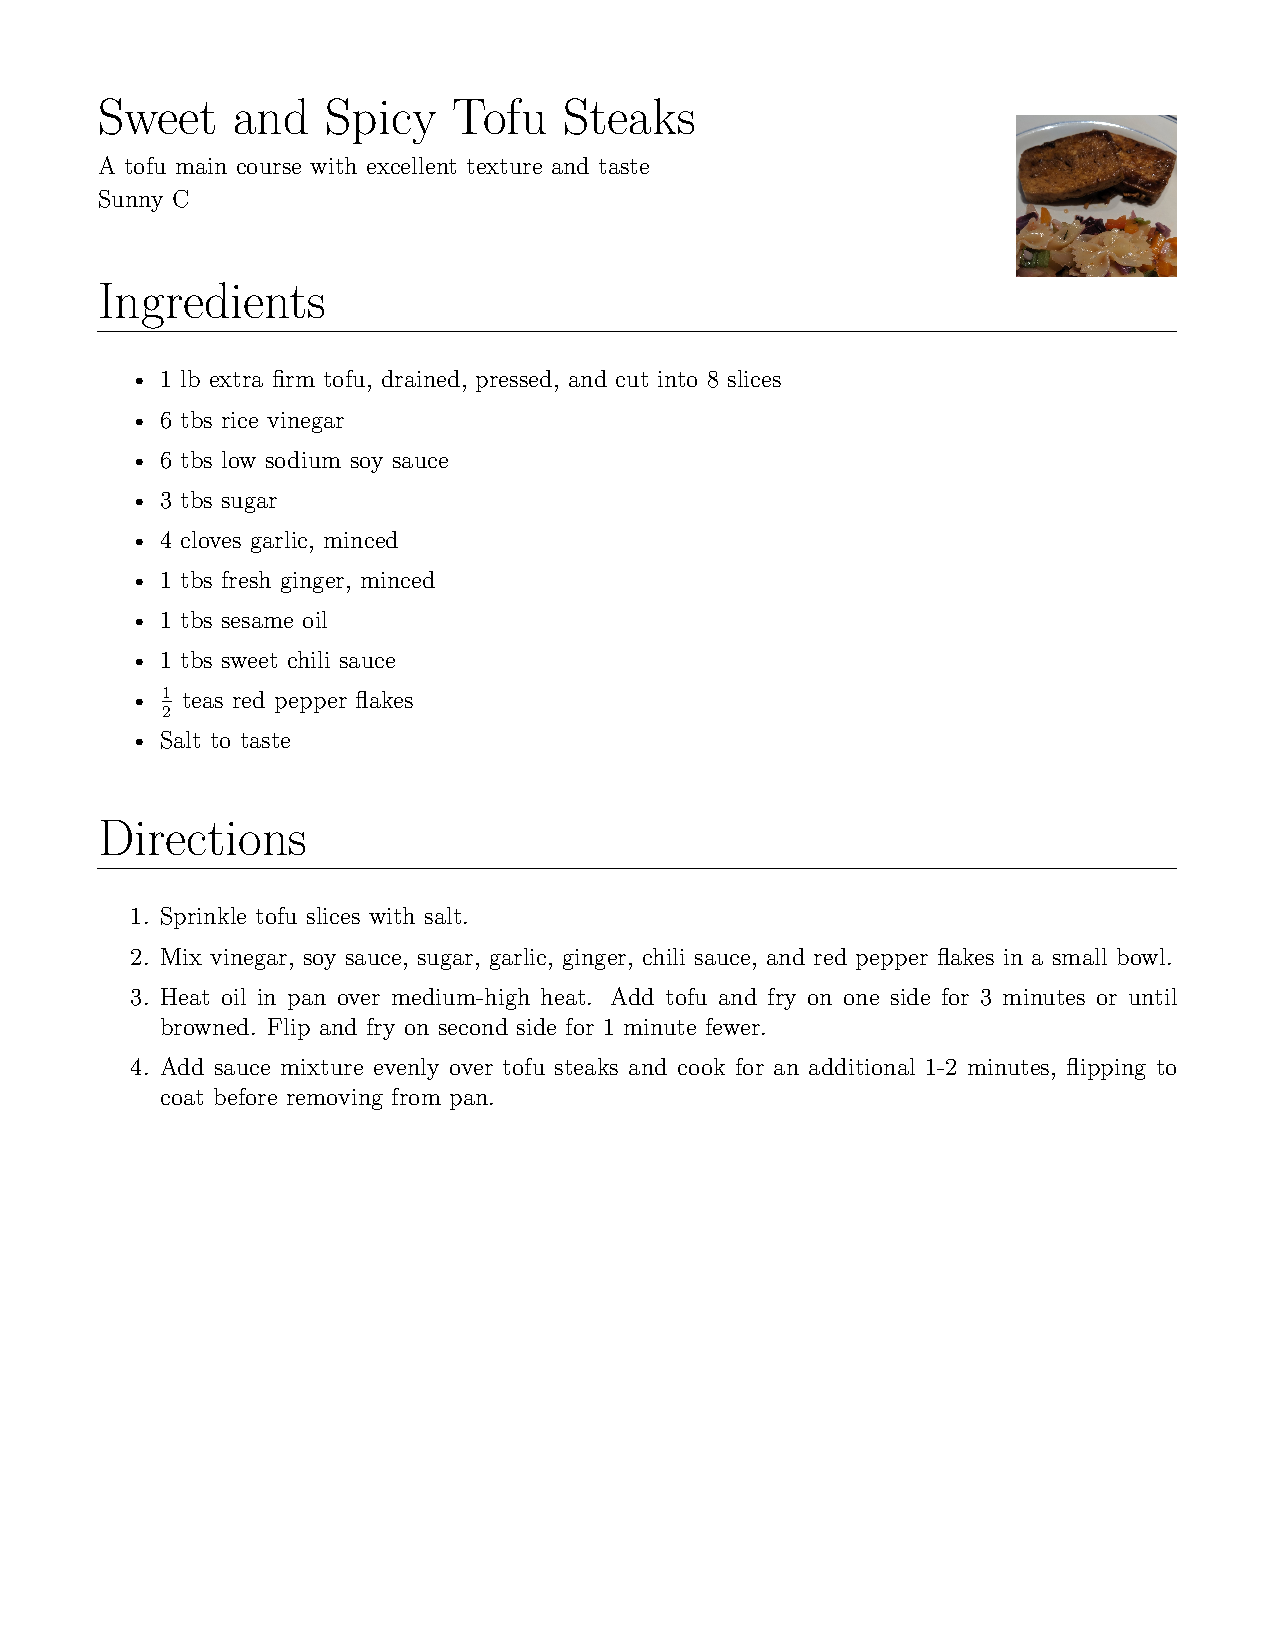
\includegraphics[width=0.15\textwidth]{sweet-and-spicy-tofu-steaks}}}\end{floatingfigure}\begin{huge}Sweet and Spicy Tofu Steaks\end{huge}\newline\vspace{-2.5mm}\newline\renewcommand{\arraystretch}{1.1}\begin{tabular*}{\textwidth}{@{\extracolsep{\fill}}lr}A tofu main course with excellent texture and taste\\Sunny C\end{tabular*}\newline\vspace{10mm}\newline\begin{huge}Ingredients\end{huge}\\\rule[2.8mm]{\textwidth}{.1pt}\vspace{-3mm}\begin{itemize}\item 1 lb extra firm tofu, drained, pressed, and cut into 8 slices\item 6 tbs rice vinegar\item 6 tbs low sodium soy sauce\item 3 tbs sugar\item 4 cloves garlic, minced\item 1 tbs fresh ginger, minced\item 1 tbs sesame oil\item 1 tbs sweet chili sauce\item $\frac{1}{2}$ teas red pepper flakes\item Salt to taste\end{itemize}\vspace{7mm}\begin{huge}Directions\end{huge}\\\rule[2.8mm]{\textwidth}{.1pt}\vspace{-3mm}\begin{enumerate}\item Sprinkle tofu slices with salt.\item Mix vinegar, soy sauce, sugar, garlic, ginger, chili sauce, and red pepper flakes in a small bowl.\item Heat oil in pan over medium-high heat. Add tofu and fry on one side for 3 minutes or until browned. Flip and fry on second side for 1 minute fewer.\item Add sauce mixture evenly over tofu steaks and cook for an additional 1-2 minutes, flipping to coat before removing from pan.\end{enumerate}\end{document}